\subsubsection{Package com.sirius.sequenziatore.server.presenter.user}
\begin{figure}[H] \centering 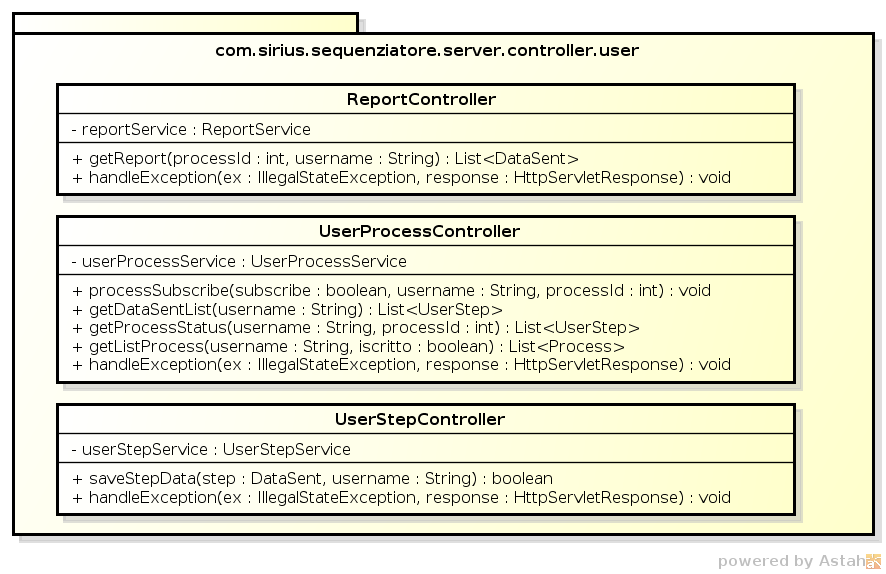
\includegraphics[width=%
\textwidth]
{./classi/server/controlleruser.png} \caption{Diagramma package - \texttt{com.sirius.sequenziatore.server.controller.user}}
\end{figure}
\paragraph{UserStepController}%----------------------------------------------------------------%
\begin{figure}[H] \centering 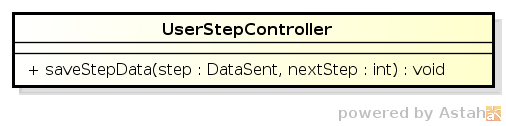
\includegraphics[width=%
\textwidth]
{./classi/server/userstepcontroller.png} \caption{Diagramma classe - \texttt{UserStepController}}
\end{figure}
\begin{itemize}
	\item \textbf{Descrizione: } Questa classe gestisce la ricezione dei dati di un passo inviati da un utente tramite una richiesta di tipo \textit{POST}, tale passo dovrà essere inserito nel database, ponendo attenzione se è un passo che richiede approvazione o meno;
	\item \textbf{Mappatura base: } \textit{\slash stepdata\slash user}
	\item \textbf{Relazioni con altri componenti: }
	La classe utilizzerà le seguenti classi:
	\begin{itemize}
		\item \texttt{com.sirius.sequenziatore.server.model.DataSent;}
		\item \texttt{com.sirius.sequenziatore.server.service.UserStepService;}
	\end{itemize}
	\item \textbf{Attributi: }\begin{itemize}
				\item \texttt{-UserStepService userStepService}.
	\end{itemize}
	\item \textbf{Metodi: }\begin{itemize}
					\item \texttt{+boolean saveStepData(DataSent step,String username):}\\
					questo metodo gestisce una richiesta \textbf{POST} da un utente, riceve i dati inerenti a un passo e affida al service l' incarico di salvare tali dati, in caso di errore lancia un' eccezione; 
					\item \texttt{+void handleException(IllegalStateException,HttpServletResponse response)}:\\
					 questo metodo è un gestore delle eccezioni e sarà incaricato di lanciare al client un errore 409.
				\end{itemize}
\end{itemize}
\paragraph{UserProcessController}%----------------------------------------------------------------%
\
\begin{figure}[H] \centering
\includegraphics[trim=0cm 0.8cm 0cm 0cm,clip=true,scale=0.75]%
{./classi/server/userprocesscontroller.png} \caption{Diagramma classe - \texttt{UserProcessController}}
\end{figure}
\begin{itemize}
	\item \textbf{Descrizione: } Questa classe permette all' utente varie operazioni, innanzitutto l' iscrizione ad un processo, poi restituisce il passo a cui è arrivato e il suo stato per tale processo e infine fornisce una lista di processi con tutti i processi a cui si può iscrivere e i processi per i quali può chiedere di fare il \textit{report};
	\item \textbf{Mappatura base: } \textit{\slash user\slash \{username\}}
	\item \textbf{Relazioni con altri componenti: }
	La classe utilizzerà le seguenti classi:
	\begin{itemize}
		\item \texttt{com.sirius.sequenziatore.server.model.Process;}
		\item \texttt{com.sirius.sequenziatore.server.model.UserStep;}
		\item \texttt{com.sirius.sequenziatore.server.model.ProcessDao;}
		\item \texttt{com.sirius.sequenziatore.server.model.StepDao;}
		\item \texttt{com.sirius.sequenziatore.server.service.UserProcessService;}
	\end{itemize}
	\item \textbf{Attributi: }\begin{itemize}
				\item \texttt{-UserProcessService userProcessService}.
	\end{itemize}
	\item \textbf{Metodi: }\begin{itemize}
					\item \texttt{+boolean processSubscribe(boolean subscribe,String username,int processId)}:\\
					questo metodo mappa su \textit{\slash subscribe\slash \{processid\}} e gestisce una richiesta di tipo \textbf{POST} incaricando  il service di iscrivere l' utente al processo voluto;
					\item \texttt{+List<UserStep> getProcessStatus(String username,int processId)}:\\
					questo metodo mappa su \textit{\slash subscribe\slash \{processid\}} e gestisce una richiesta \textbf{GET} che restituisce all' utente il proprio status per tale processo, restituendo il passo o i passi che può eseguire e quanti passi ha completato del processo;
					\item \texttt{+List<Process> getListProcess(String username,boolean iscritto)}:\\
					questo metodo mappa su \textit{\slash processlist} e gestisce una richiesta di tipo \textbf{GET} andando e restituire una lista di processi che contiene tutti i processi  a cui è iscritto e quelli a cui si può iscrivere;
					\item \texttt{+List<UserStep> getDataSentList(String username):}\\
					questo metodo gestisce una richiesta di tipo \textbf{GET} e restituisce all' utente il proprio status per tale processo.
					\item \texttt{+void handleException(IllegalStateException,HttpServletResponse response)}:\\
					 questo metodo è un gestore delle eccezioni e sarà incaricato di lanciare al client un errore 409.
				\end{itemize}
\end{itemize}
\paragraph{ReportController}%----------------------------------------------------------------%
\
\begin{figure}[H] \centering
\includegraphics[trim=0cm 0.8cm 0cm 0cm,clip=true,scale=0.75]%
{./classi/server/reportcontroller.png} \caption{Diagramma classe - \texttt{ReportController}}
\end{figure}
\begin{itemize}
	\item \textbf{Descrizione: } Questa classe fornirà al client tutti i dati necessari per creare il report di un utente per un certo processo;
	\item \textbf{Mappatura base: } \textit{\slash report\slash \{username\}\slash \{processid\}}
	\item \textbf{Relazioni con altri componenti: }
	La classe utilizzerà le seguenti classi:
	\begin{itemize}
		\item \texttt{com.sirius.sequenziatore.server.model.DataSent;}
		\item \texttt{com.sirius.sequenziatore.server.service.ReportService;}
	\end{itemize}
	\item \textbf{Attributi: }\begin{itemize}
				\item \texttt{-ReportService reportService}.
	\end{itemize}
	\item \textbf{Metodi: }\begin{itemize}
					\item \texttt{+List<DataSent> getReportData(DataSent step,String username):}\\
					questo metodo gestisce una richiesta di tipo \textbf{GET} e fornirà tutti i dati inseriti da un utente per un certo processo;
				\end{itemize}
\end{itemize}